\section{Replace busy-wait techniques using the \texttt{SysTick} timer}

Using a busy-wait technique to delay for a certain amount of time is not efficient.
Wasting \enquote{expensive} CPU cycles should be avoided whenever possible.
This is where hardware timers comes in.
Hardware timers decrement or increment a given value at a certain frequency and generates a signal if the value reached a treshold (this could be in the form of underflow or overflow aswell as reaching a certain value where 0 is the most common one).
This chapter describes the \texttt{SysTick} hardware timer.

\subsection{\texttt{SysTick} timer and interrupt using DRM}
\label{subsec:systick_drm}

As mentioned in the previous section, when one uses the DRM programming technique it is important that the programmer knows the microcontroller really well.
Understanding the different Special Function Registers (SFR) related to the hardware module one wants to use is a consequence.
The three SFR related to \texttt{SysTick} are described below.

\begin{figure}[H]
\centering

\begin{bytefield}[endianness=big, bitwidth=3.0em]{30}
\bitheader[lsb=2]{16-31} \\
    \bitbox{15}{\tiny Reserved} &
    \colorbitbox{celadon}{1}{\tiny COUNT} \\ [3ex]
\bitheader[lsb=-14]{0-15} \\
    \bitbox{13}{\tiny Reserved}
    \colorbitbox{celadon}{1}{\tiny CLK\_SRC}
    \colorbitbox{celadon}{1}{\tiny INTEN}
    \colorbitbox{celadon}{1}{\tiny ENABLE}
\end{bytefield}

\caption{\texttt{STCTRL} register for the CC3220s}
\label{fig:stctrl}

\end{figure}

First, there is \texttt{STCTRL} (\texttt{SysTick} Control Register) which enables the \texttt{SysTick} features \cite{CC3220s_reference_manual}.
Bit 0 (Figure \ref{fig:stctrl}) enables the \texttt{SysTick} module if this bit is set or disables the \texttt{SysTick} module if this bit is cleared.
The \texttt{SysTick} module will generate an interrupt only if bit 1 is set.
The clock source fed into the \texttt{SysTick} module can be the system clock if bit 3 is set or a precision internal oscillator if bit 3 is cleared \cite{CC3220s_reference_manual}.


\begin{figure}[H]
\centering

\begin{bytefield}[endianness=big, bitwidth=3.0em]{30}
\bitheader[lsb=2]{16-31} \\
    \bitbox{8}{\tiny Reserved} &
    \colorbitbox{celadon}{8}{\tiny RELOAD} \\ [3ex]
\bitheader[lsb=-14]{0-15} \\
    \colorbitbox{celadon}{16}{\tiny RELOAD}
\end{bytefield}

\caption{\texttt{STRELOAD} register for the CC3220s}
\label{fig:streload}

\end{figure}

Second, there is \texttt{STRELOAD} register (Figure \ref{fig:streload}) which stores the constant that should be loaded to the \texttt{STCURRENT} register if the previous value reached value 0.
One should keep in mind that if the desired behaviour is an interrupt or a flag every $x$ ticks, one should store $x - 1$ ticks in this register.
This is because the \texttt{RELOAD} value is copied to \texttt{STCURRENT} current register if 0 is reached (so not one tick after zero).

\begin{figure}[H]
\centering

\begin{bytefield}[endianness=big, bitwidth=3.0em]{30}
\bitheader[lsb=2]{16-31} \\
    \bitbox{8}{\tiny Reserved} &
    \colorbitbox{celadon}{8}{\tiny CURRENT} \\ [3ex]
\bitheader[lsb=-14]{0-15} \\
    \colorbitbox{celadon}{16}{\tiny CURRENT}
\end{bytefield}

\caption{\texttt{STCURRENT} register for the CC3220s}
\label{fig:stcurrent}

\end{figure}

The last register is the \texttt{STCURRENT} register.
This register holds the current value being decremented.
An important detail is that the \texttt{CURRENT} field is write-clear behaviour.
This means that writing any value to this field clears the register and the \texttt{COUNT} bit of the \texttt{STCTRL} register \cite{CC3220s_reference_manual}.

\newpage
\begin{lstlisting}[style=CStyle, caption={Toggling LEDs according to Table \ref{tab:led_scheme} using DRM programming technique}, captionpos=b, label={lst:led_systick_drm}, escapechar=@]
#include <stdint.h>
#include <stddef.h>
#include "register_def.h"

#include "inc\hw_memmap.h"
#include "inc\hw_gpio.h"
#include "inc\hw_apps_rcm.h"
#include "inc\hw_ocp_shared.h"

static volatile _Bool flag_led_update;  @\label{line:drm_systick_flag}@

void SysTickHandler()   @\label{line:drm_systick_irq}@
{
    static int tick_count = 0;
    flag_led_update = tick_count == 1000 ? 1 : 0;   @\label{line:drm_systick_set_flag}@
    tick_count = (tick_count+1) % (1000 + 1);       @\label{line:drm_systick_inc}@
}

int main(void)
{

    /* Init SysTick */
    HWREG(NVIC_ST_CTRL) = 0x00;         // Disable SysTick during setup     @\label{line:drm_systick_disable}@
    HWREG(NVIC_ST_RELOAD) = 79999;      // Get every millisecond an interrupt (80 000 - 1)  @\label{line:drm_systick_reload}@
    HWREG(NVIC_ST_CURRENT) = 0x00;      // Clear any flags and set current value to 0       @\label{line:drm_systick_current}@
    HWREG(NVIC_ST_CTRL) = 0x07;         // Enable SysTick, Enable interrupt, CLK_SRC = System clock @\label{line:drm_systick_enabe}@

    /* Init LEDS */
    HWREG(ARCM_BASE + APPS_RCM_O_GPIO_A_CLK_GATING) = 0x01;     @\label{line:drm_systick_gpio_enable}@

    HWREG(OCP_SHARED_BASE + OCP_SHARED_O_GPIO_PAD_CONFIG_9) = 0x60; @\label{line:drm_systick_pad_one}@
    HWREG(OCP_SHARED_BASE + OCP_SHARED_O_GPIO_PAD_CONFIG_10) = 0x60;
    HWREG(OCP_SHARED_BASE + OCP_SHARED_O_GPIO_PAD_CONFIG_11) = 0x60;@\label{line:drm_systick_pad_three}@

    HWREG(GPIOA1_BASE + GPIO_O_GPIO_DIR) = 0x0E;            @\label{line:drm_systick_dir}@
    HWREG(GPIOA1_BASE + GPIO_O_GPIO_DATA + (0x0E << 2)) = 0x00; @\label{line:drm_systick_init_data}@

    unsigned int index = 0;

    while(1)
    {
        if(!flag_led_update)        @\label{line:drm_systick_is_update}@
            continue;               @\label{line:drm_systick_continue}@

        HWREG(GPIOA1_BASE + GPIO_O_GPIO_DATA + (0x0E << 2)) = index;    @\label{line:drm_systick_set_led}@
        index = (index + 1) % 16;                                       @\label{line:drm_systick_inc_index}@
        flag_led_update = 0;                                            @\label{line:drm_systick_clear_flag}@
    }

    return 0;
}
\end{lstlisting}

Listing \ref{lst:led_systick_drm} shows the programming source code to toggle the LEDs using the \texttt{SysTick} timer module to delay the correct amount of time.
Line \ref{line:drm_systick_flag} contains a shared variable which is used as a flag. If this variable is set the main loop should toggle the LEDs in the next row in Table \ref{tab:led_scheme}. If this variable is not set then the main loop has to do nothing.
Line \ref{line:drm_systick_irq} is the entry point for the \texttt{SysTick} event handler.
Every time a \texttt{SysTick} interrupt occurs this piece of event handler code is executed.
There should be a delay of 1 second between every row in Table \ref{tab:led_scheme}. Since the \texttt{SysTick} interrupt is executed every 1 millisecond the code should execute the \texttt{SysTick} handler 1000 times before updating the shared variable.
\texttt{tick\_count} takes care of that. This static variable does not lose its content between two execution runs of the event handler.
Every interrupt this variable is incremented (Line \ref{line:drm_systick_inc}) and when its incremented 1000 times the shared variable is set (Line \ref{line:drm_systick_set_flag}). 

\newpage
After booting, the first thing done is disabling the \texttt{SysTick} module (Line \ref{line:drm_systick_disable}) by setting all bits in the \texttt{STCTRL} register to 0 (including the \texttt{\scriptsize ENABLE} bit).
Then it loads the reset value $80 000 - 1$ into the \texttt{STRELOAD} register (Line \ref{line:drm_systick_reload}) and clears the current value and any flags already set (Line \ref{line:drm_systick_current}).
\texttt{\scriptsize ENABLE}, \texttt{\scriptsize INTEN} and \texttt{\scriptsize CLK\_SRC} bits in the \texttt{STCTRL} register (Figure \ref{fig:stctrl}) are set by writing $00000111_2$ or $0x07_{16}$ to this register.
From this point in the code the \texttt{SysTick} module is enabled and decrementing.\newline

What now follows is a description of the main code. 
This is almost identical to the code described in Section \ref{subsec:led_drm}.
The registers related to GPIO can be found in that section aswell.
Line \ref{line:drm_systick_gpio_enable} in Listing \ref{lst:led_systick_drm} enables the GPIOA peripheral.
Line \ref{line:drm_systick_pad_one} up to and including Line \ref{line:drm_systick_pad_three} configures the behaviour of GPIO pin 9, GPIO pin 10 and GPIO pin 11. Those pins are configured to have a maximum current usage of 6 mA.
Line \ref{line:drm_systick_dir} configures GPIO pin 9, GPIO pin 10 and GPIO pin 11  as an output pin.
Line \ref{line:drm_systick_init_data} turns those GPIO pins off according to first row of Table \ref{tab:led_scheme}. \newline

The following code is executed in an endless loop.
Line \ref{line:drm_systick_is_update} and Line \ref{line:drm_systick_continue} were not present in Section \ref{subsec:led_drm}.
Line \ref{line:drm_systick_is_update} checks if the shared variable \texttt{flag\_led\_update} is set by the \texttt{SysTick} event handler. It it is not Line \ref{line:drm_systick_continue} is executed and the check will be executed again.
If it is set then Line \ref{line:drm_systick_set_led} up to and including Line \ref{line:drm_systick_clear_flag} will be executed.
Line \ref{line:drm_systick_set_led} writes the new sequence of LEDs to the GPIO pins.
Line \ref{line:drm_systick_inc_index} increments the sequence so the next row in Table \ref{tab:led_scheme} will be set next time the shared variable is set.
Line \ref{line:drm_systick_clear_flag} clears the flag so the next iteration of the loop won't update the LEDs again.

The reader may wonder how the microcontroller knows which function should be executed on a \texttt{SysTick} interrupt.
This is done using the vector table. This vector table contains different function names for different kind of interrupts (Listing \ref{lst:systick_vector_table_min}).
Because the function definition \texttt{SysTickHandler} is in \texttt{main.c} we declare it as extern so the compiler will not fail and the linker will search for the external references in a later stage of the compilation process.

\begin{lstlisting}[style=CStyle, caption={Part of \texttt{cc3220\_startup\_ccs.c} which contains a part of the vector table}, captionpos=b, label={lst:systick_vector_table_min}, escapechar=@]
......
......
extern void SysTickHandler();
......
......

void (* const resetVectors[43])(void) =
{
    (void (*)(void))((unsigned long)&__STACK_END),
                                         // The initial stack pointer
    resetISR,                            // The reset handler
    nmiISR,                              // The NMI handler
    faultISR,                            // The hard fault handler
    defaultHandler,                      // The MPU fault handler
    busFaultHandler,                     // The bus fault handler
    defaultHandler,                      // The usage fault handler
    0,                                   // Reserved
    0,                                   // Reserved
    0,                                   // Reserved
    0,                                   // Reserved
    defaultHandler,                     // SVCall handler
    defaultHandler,                      // Debug monitor handler
    0,                                   // Reserved
    defaultHandler,                      // The PendSV handler
    SysTickHandler,                      // The SysTick handler
    defaultHandler,                      // GPIO Port A0
    defaultHandler,                      // GPIO Port A1
    defaultHandler,                      // GPIO Port A2
    defaultHandler,                      // GPIO Port A3
    ......
    ......
}

\end{lstlisting}

For more information about exception, interrupts and the vector table, see Appendix \ref{subsec:appendix_vector}.

\newpage
\subsection{\texttt{SysTick} timer and interrupt using Driverlib}

The code listings presented in the previous subsection can also be converted using Driverlib.
This converted code using Driverlib can be seen in Listing \ref{lst:led_systick_driverlib}
Quite some code in Listing \ref{lst:led_systick_driverlib} has not been changed compared to Listing \ref{lst:led_systick_drm}.
The shared variable \texttt{flag\_led\_update} in Line \ref{line:driverlib_systick_shared} is still there.
The \texttt{SysTick} event handler in Line \ref{line:driverlib_systick_handler} is identical to the \texttt{SysTick} event handler in Line \ref{line:drm_systick_irq} of Listing \ref{lst:led_systick_drm}.
In fact the behaviour of the code is exactly the same as the one generated by Listing \ref{lst:led_systick_drm}.
However, because Driverlib is used some code changed.\newline

Line \ref{line:driverlib_systick_disable} disables the \texttt{SysTick} module. 
Line \ref{line:driverlib_systick_period} sets the period (every millisecond an interrupt is generated).
Please note that using DRM the value 79 999 has to be loaded in the \texttt{STRELOAD} register.
By using an abstraction layer such as Driverlib we do not have to take this into account.
Line \ref{line:driverlib_systick_interrupt} will register the function \texttt{SysTickHandler} to be called once a SysTick event occurs.
Line \ref{line:driverlib_systick_enable} enables the \texttt{SysTick} module.
Line \ref{line:driverlib_systick_enable_gpio} enables the GPIO A1 module (where GPIO 9, GPIO 10 and GPIO 11 are connected to).
Line \ref{line:driverlib_systick_padconfig1} up to and including Line \ref{line:driverlib_systick_padconfig3} configures the characteristics of GPIO 9, GPIO 10 and GPIO 11. Those pins can not use more than 2 mA.
Line \ref{line:driverlib_systick_output1} up to and including Line \ref{line:driverlib_systick_output3} configures GPIO 9, GPIO 10 and GPIO 11 as output pins.\newline
The shared varible \texttt{flag\_led\_update} is polled in a loop and when it is set by the \texttt{SysTickHandler} it will write the next LED sequence of Table \ref{tab:led_scheme} to the three GPIO pins (line \ref{line:driverlib_systick_writepin}), update the variable \texttt{switcher} so the next sequence will be written once \texttt{flag\_led\_update} is set again (Line \ref{line:driverlib_systick_inc}) and the shared variable \texttt{flag\_led\_update} is cleared so the next loop iteration will not enter Line \ref{line:driverlib_systick_writepin} again. \newline

Currently the main program polls the shared variable \texttt{flag\_led\_update} to see whether if it has to update the LEDs.
Using this technique does not solve our issue when we started using the \texttt{SysTick} module.
Busy-wait or polling should be avoided as much as possible and by using the \texttt{SysTick} module the current implementation polls on the shared variable \texttt{flag\_led\_update}.
A really simple solution is to turn the microprocessor in a \enquote{sleep} mode.
During such mode no instructions are fetched and executed thus less power is consumed.
There is an ARM assembly instruction \texttt{WFI} (Wait For Interrupt) which turns the microprocessor in a sleep mode untill an interrupt occurs.
This is ideal for such a simple program as Listing \ref{lst:led_systick_driverlib} because no other useful work can be done untill the \texttt{SysTickHandler} eventually sets the shared variable.
Line \ref{line:driverlib_systick_ass1} uses the DRM (like) technique by executing this Assembly instruction.
One could also use Driverlib to enter the wait for interrupt state (Line \ref{line:driverlib_systick_ass2}).

\newpage
\begin{lstlisting}[style=CStyle, caption={Toggling LEDs according to Table \ref{tab:led_scheme} using Driverlib}, captionpos=b, label={lst:led_systick_driverlib}, escapechar=@]
#include <stdint.h>
#include <stddef.h>
#include "register_def.h"

#include <gpio.h>
#include <pin.h>
#include <prcm.h>
#include <systick.h>

static volatile _Bool flag_led_update;  @\label{line:driverlib_systick_shared}@

void SysTickHandler()       @\label{line:driverlib_systick_handler}@
{
    static int tick_count = 0;
    flag_led_update = tick_count == 1000 ? 1 : 0;
    tick_count = (tick_count+1) % (1000 + 1);
}

int main(void)
{
    SysTickDisable();       @\label{line:driverlib_systick_disable}@
    SysTickPeriodSet(80000);    @\label{line:driverlib_systick_period}@
    SysTickIntRegister(SysTickHandler); @\label{line:driverlib_systick_interrupt}@
    SysTickIntEnable();     @\label{line:driverlib_systick_enable_interrupt}@
    SysTickEnable();        @\label{line:driverlib_systick_enable}@

    PRCMPeripheralClkEnable(PRCM_GPIOA1 ,PRCM_RUN_MODE_CLK);    @\label{line:driverlib_systick_enable_gpio}@

    PinTypeGPIO(PIN_64, PIN_STRENGTH_2MA, false);   /* Red LED is push-pull */      @\label{line:driverlib_systick_padconfig1}@
    PinTypeGPIO(PIN_01, PIN_STRENGTH_2MA, false);   /* Yellow LED is push-pull */   @\label{line:driverlib_systick_padconfig2}@
    PinTypeGPIO(PIN_02, PIN_STRENGTH_2MA, false);   /* Green LED is push-pull */    @\label{line:driverlib_systick_padconfig3}@

    GPIODirModeSet(GPIOA1_BASE, GPIO_PIN_2, GPIO_DIR_MODE_OUT);                     @\label{line:driverlib_systick_output1}@
    GPIODirModeSet(GPIOA1_BASE, GPIO_PIN_3, GPIO_DIR_MODE_OUT);                     @\label{line:driverlib_systick_output2}@
    GPIODirModeSet(GPIOA1_BASE, GPIO_PIN_1, GPIO_DIR_MODE_OUT);                     @\label{line:driverlib_systick_output3}@

    GPIOPinWrite(GPIOA1_BASE, GPIO_PIN_2, ~GPIO_PIN_2);  /* Turn yellow LED off */
    GPIOPinWrite(GPIOA1_BASE, GPIO_PIN_3, ~GPIO_PIN_3);  /* Turn green LED off */
    GPIOPinWrite(GPIOA1_BASE, GPIO_PIN_1, ~GPIO_PIN_1);  /* Turn red LED off */

    unsigned int switcher = 0;

    while(1)
    {
        if(flag_led_update)
        {
            GPIOPinWrite(GPIOA1_BASE, GPIO_PIN_1 | GPIO_PIN_2 | GPIO_PIN_3, switcher);  @\label{line:driverlib_systick_writepin}@
            switcher = (switcher + 1) % 16;                                             @\label{line:driverlib_systick_inc}@
            flag_led_update = 0;                                                        @\label{line:driverlib_systick_reset}@
        }

        // __asm("     WFI");   /* Uncomment to meet assignment 2.4 */              @\label{line:driverlib_systick_ass1}@
        // PRCMSleepEnter();    /* Uncomment to meet assignment 2.5 */              @\label{line:driverlib_systick_ass2}@
    }

    return 0;
}
\end{lstlisting}

\newpage
\subsection{Traffic light using Driverlib}

A very simple static scheduler can be implemented to control a traffic light.
The characteristics of the different coloured lights can be seen in Table \ref{tab:led_trafficlight}.

\begin{table}[H]
    \centering
    \begin{tabular}{|c|c|}
        \hline
        \textcolor{darkpink}{\textit{Colour}} & \textcolor{darkpink}{\textit{Time bright (s)}}\\
        \hline
        Red & 5 \\
        \hline
        Yellow & 1 \\
        \hline
        Green & 4 \\
        \hline
    \end{tabular}
            
    \label{tab:led_trafficlight}
    \caption{Timing characteristics for the different colours of the traffic light}
\end{table}

The code is split up into two parts to keep the overview.
The first part defines a few datatypes, global variables and two functions (where one is an event handler).
Line \ref{line:ss_state} in Listing \ref{lst:static_scheduler_1} defines a datatype \texttt{state\_t} which is a datatype to hold the current LED colour to lit.
Line \ref{line:ss_state_var} makes one global variable (\texttt{state}) of the just created datatype \texttt{state\_t} to hold the current LED to lit.
Line \ref{line:ss_ticks} makes a global variable \texttt{ticks} which is used in the \texttt{SysTickHandler} to increment (Line \ref{line:ss_inc_ticks}).
Those ticks are used to determine if the amount of time a certain LED has lit is expired.
If it has not expired then the microprocessor enters a sleep mode (Line \ref{line:ss_sleep}).
However, if the time a certain LED has expired the \texttt{tick} variable is reset (Line \ref{line:ss_reset_ticks}) and the next state is set (Line \ref{line:ss_new_state}).
The different states are explained in part two of the static scheduler.

\begin{lstlisting}[style=CStyle, caption={First part of the static scheduler which defines some data types and states}, captionpos=b, label={lst:static_scheduler_1}, escapechar=@]
#include <stdint.h>
#include <stddef.h>
#include "register_def.h"

#include <gpio.h>
#include <pin.h>
#include <prcm.h>
#include <systick.h>

typedef enum {
    STATE_RED,
    STATE_YELLOW,
    STATE_GREEN
} state_t; @\label{line:ss_state}@

static volatile state_t state; @\label{line:ss_state_var}@
static volatile unsigned int tick;  @\label{line:ss_ticks}@

void SysTickHandler()
{
    tick++;                     @\label{line:ss_inc_ticks}@
}

void next_state(state_t newState, unsigned int delayInSeconds)
{
    while((tick/1000) < delayInSeconds)
        PRCMSleepEnter();   @\label{line:ss_sleep}@

    tick = 0;               @\label{line:ss_reset_ticks}@
    state = newState;           @\label{line:ss_new_state}@
}

\end{lstlisting}


\newpage
The second part of the static scheduler can be found in Listing \ref{lst:static_scheduler_2}.
Line \ref{line:ss_not_explained1} up to and including Line \ref{line:ss_not_explained2} will not be explained again because those lines have been explained in the previous subsection.
Explaining them again would be redundant.
The defaultk state is that the red LED is lit (Line \ref{line:ss_default_state}).
There is no particular reason why the initial behaviour is that the red LED is lit.
The reader is free to change the initial LED colour.
A kind of state machine has been implemented to switch between LEDs (Line \ref{line:ss_sm_1} up to and including Line \ref{line:ss_sm_2}).
In a certain state the LEDs are written with a certain pattern for that particular state using the \texttt{GPIOPinWrite} function.
The interesting part comes after setting the LEDs.
A function call to \texttt{next\_state} is made with the first parameter being the next state that should be entered and the second parameter howmuch seconds this current state should last.
\texttt{next\_state} uses the \texttt{ticks} global variable to keep track if the current state should be changed to the next state.
If the current state has not been up for the desired amount of seconds the microprocessor enters the sleep mode.
After an interrupt and the \texttt{SysTickHandler} increments \texttt{ticks} the function \texttt{next\_state} will test again if the current state has been up for the desired amount.
This goes on and on untill the desired amount of seconds has been reached and the next state is set.

\begin{lstlisting}[style=CStyle, caption={Second part of the static scheduler}, captionpos=b, label={lst:static_scheduler_2}, escapechar=@]
int main(void)
{
    SysTickDisable();               @\label{line:ss_not_explained1}@
    SysTickPeriodSet(80000);
    SysTickIntRegister(SysTickHandler);
    SysTickIntEnable();
    SysTickEnable();

    PRCMPeripheralClkEnable(PRCM_GPIOA1 ,PRCM_RUN_MODE_CLK);

    PinTypeGPIO(PIN_64, PIN_STRENGTH_2MA, false);   /* Red LED is push-pull */
    PinTypeGPIO(PIN_01, PIN_STRENGTH_2MA, false);   /* Yellow LED is push-pull */
    PinTypeGPIO(PIN_02, PIN_STRENGTH_2MA, false);   /* Green LED is push-pull */

    GPIODirModeSet(GPIOA1_BASE, GPIO_PIN_2, GPIO_DIR_MODE_OUT);
    GPIODirModeSet(GPIOA1_BASE, GPIO_PIN_3, GPIO_DIR_MODE_OUT);
    GPIODirModeSet(GPIOA1_BASE, GPIO_PIN_1, GPIO_DIR_MODE_OUT);

    GPIOPinWrite(GPIOA1_BASE, GPIO_PIN_2, ~GPIO_PIN_2);  /* Turn yellow LED off */
    GPIOPinWrite(GPIOA1_BASE, GPIO_PIN_3, ~GPIO_PIN_3);  /* Turn green LED off */
    GPIOPinWrite(GPIOA1_BASE, GPIO_PIN_1, ~GPIO_PIN_1);  /* Turn red LED off */     @\label{line:ss_not_explained2}@

    state = STATE_RED;      @\label{line:ss_default_state}@

    while(1)
    {
        switch(state)       @\label{line:ss_sm_1}@
        {
        case STATE_RED:
            GPIOPinWrite(GPIOA1_BASE, GPIO_PIN_1 | GPIO_PIN_2 | GPIO_PIN_3, 0x02);
            next_state(STATE_YELLOW, 5);
            break;
        case STATE_YELLOW:
            GPIOPinWrite(GPIOA1_BASE, GPIO_PIN_1 | GPIO_PIN_2 | GPIO_PIN_3, 0x04);
            next_state(STATE_GREEN, 1);
            break;
        case STATE_GREEN:
            GPIOPinWrite(GPIOA1_BASE, GPIO_PIN_1 | GPIO_PIN_2 | GPIO_PIN_3, 0x08);
            next_state(STATE_RED, 4);
            break;
        }                   @\label{line:ss_sm_2}@

    }

    return 0;
}
\end{lstlisting}

\newpage
\subsection{Verification of the timing specifications}


\begin{figure}[H]
    \centering

    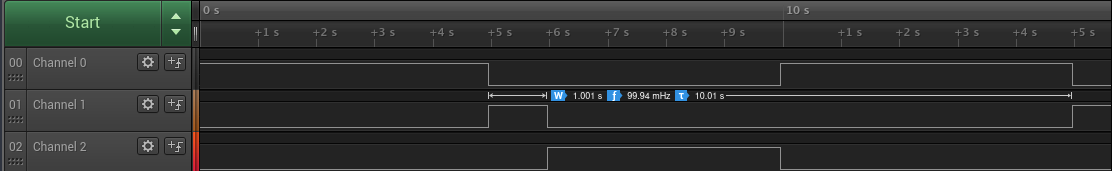
\includegraphics[scale=0.43]{img/yellow.png}

    \caption{The yellow LED is lit for 1.001 seconds}
    \label{fig:yellow}

\end{figure}

\begin{figure}[H]
    \centering

    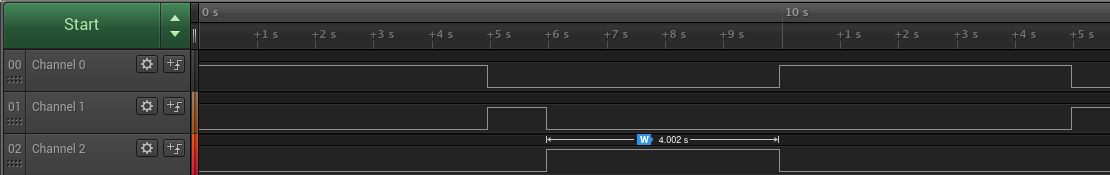
\includegraphics[scale=0.43]{img/green.png}

    \caption{The green LED is lit for 4.002 seconds}
    \label{fig:green}

\end{figure}

\begin{figure}[H]
    \centering

    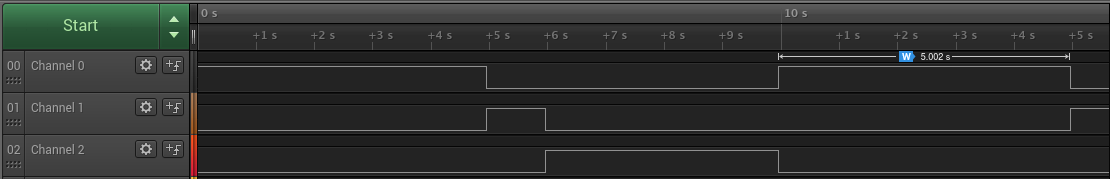
\includegraphics[scale=0.43]{img/red.png}

    \caption{The red LED is lit for 5.002 seconds}
    \label{fig:red}

\end{figure}
